\documentclass[12pt,Chicago]{uuthesis2e}
\usepackage[letterpaper]{geometry}

\let \proof    = \relax
\let \endproof = \relax
\usepackage {amsthm}
\usepackage{mathpazo}
\fourlevels
\usepackage {amsmath}
\usepackage {amssymb}
\usepackage {bm}
\usepackage {bibnames}
\usepackage {citesort}
\usepackage {graphicx}
\usepackage {graphpap}
\usepackage {longtable}
\usepackage {multirow}
\usepackage {tikz}
\usetikzlibrary {decorations.markings}
\usepackage {varioref}
\usepackage
{
    cite, 
    epsfig,
    epstopdf, 
    color, 
    float,
    subfig,
    xspace,
    tabularx,
    rotating,
    lscape,
    afterpage,
    url,
    listings,
	hhline
} 

\usepackage[ruled]{./algorithm2e}
\usepackage {uuthesis-2016-h}  % MANDATORY package
\usepackage {mythesis}

\newtheorem{Theorem}{Theorem}[chapter]
\newtheorem{Definition}{Definition}[chapter]
\newtheorem{Example}{Example}[chapter]
\newtheorem{Proposition}{Proposition}[chapter]
\newtheorem{Lemma}{Lemma}[chapter]
\newtheorem{Corollary}{Corollary}[chapter]

\title{Abstraction Models For\\ Manufacturability Aware Silicon Photonics} 
\author{Carlos Daniel Gonzalez-Campos} 
\thesistype{thesis}
\degree{Bachelor of Science}

%%%%%%%%%%%%%%%%%%%%%%%%%%%%%%%%%%%%%%%%%%%%%%%%%%%%%%%%%%%%%%%%%%%%%%%%

\chairtitle{Professor}
\committeechair{Priyank Kalla}
% \firstreader{Pierre-Emmanuel Gaillardon}
% \secondreader{Chris Myers}
% \thirdreader{Kenneth Stevens}
%\graduatedean{DAVID KIEDA}
\department{Department of Electrical and Computer Engineering}
\departmentchair{FLORIAN SOLZBACHER}

\submitdate{May 2023}
\copyrightyear{2023}
\dedication{Dedications, if any !! }

\begin{document}

%% Comment out items by inserting a percent % character
\frontmatterformat
\titlepage
\copyrightpage
%\committeeapproval
%\readingapproval
% \setcounter {page}     {2}             % UofU Thesis Office demands abstract on p. iii: start one lower
\preface{abstract} {Abstract}
\dedicationpage
\tableofcontents
\listoffigures
\listoftables
%
\maintext       % Start normal page numbering: parts and chapters follow.

\pagestyle{headings} % NEW for sample-thesis-6
%\chapter{Introduction}
\label{ch:intro1}

Lorem ipsum dolor sit amet, consectetur adipiscing elit. Duis tincidunt eros ut dictum tempor. Proin rhoncus elementum mauris, ac bibendum quam. Sed eget nisi non arcu malesuada pulvinar a at ipsum. Curabitur ante quam, aliquet id purus ac, interdum semper odio. Suspendisse potenti. Aliquam rhoncus massa consectetur faucibus condimentum. Sed euismod tellus eu mattis elementum. In nec laoreet ligula. Donec vel blandit ante. Mauris non ligula non justo venenatis rhoncus. In quis auctor ipsum, in mattis lacus. In vitae lectus sodales arcu iaculis bibendum. Fusce ornare at ex vitae ultricies.

Nullam sagittis maximus leo, sit amet dictum neque suscipit at. Proin sagittis mollis mi, at ornare ligula ornare nec. Donec et pulvinar mi. Nulla ac semper dui, id mollis ante. Nam cursus vel tellus quis maximus. Vestibulum quis nunc sit amet felis mollis facilisis sed a sapien. Sed sit amet nisi velit. Mauris tellus arcu, commodo in feugiat in, porttitor vitae urna. Vivamus in aliquet elit. Nunc quis dui massa. Morbi blandit fringilla dui et fermentum. Nulla facilisi. Aenean et dui turpis. Mauris tempor diam ac mi scelerisque lacinia.\cite{fv_graph:book}, as shown in Fig. \ref{fig:fv_graph}.

\begin{figure}[H]
    \centering
    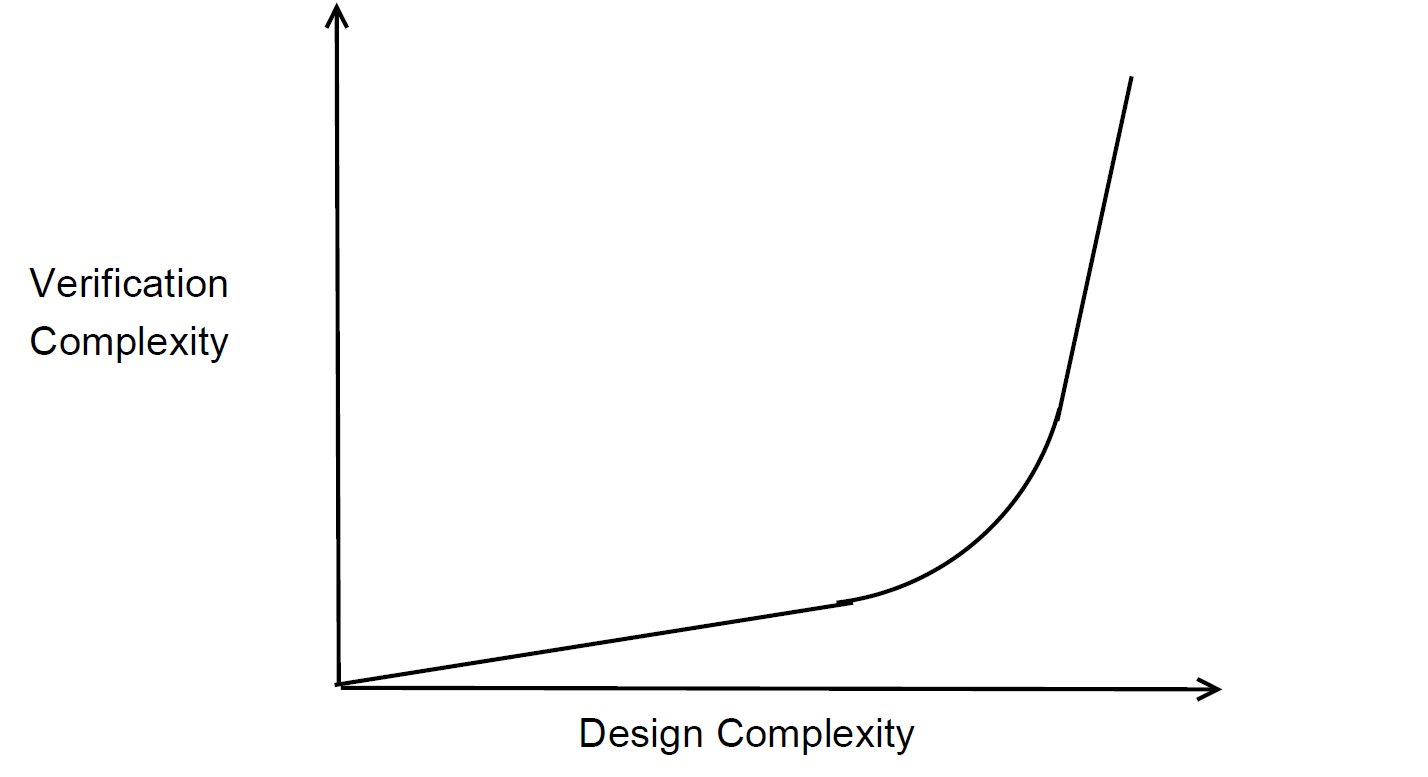
\includegraphics[scale = 0.5]{fv_graph.PNG}
    \caption{Design vs. Verification Complexity}
    \label{fig:fv_graph}
\end{figure}

\section{Hardware Design Overview}

Lorem ipsum dolor sit amet, consectetur adipiscing elit. Duis tincidunt eros ut dictum tempor. Proin rhoncus elementum mauris, ac bibendum quam. Sed eget nisi non arcu malesuada pulvinar a at ipsum. Curabitur ante quam, aliquet id purus ac, interdum semper odio. Suspendisse potenti. Aliquam rhoncus massa consectetur faucibus condimentum. Sed euismod tellus eu mattis elementum. In nec laoreet ligula. Donec vel blandit ante. Mauris non ligula non justo venenatis rhoncus. In quis auctor ipsum, in mattis lacus. In vitae lectus sodales arcu iaculis bibendum. Fusce ornare at ex vitae ultricies.

Nullam sagittis maximus leo, sit amet dictum neque suscipit at. Proin sagittis mollis mi, at ornare ligula ornare nec. Donec et pulvinar mi. Nulla ac semper dui, id mollis ante. Nam cursus vel tellus quis maximus. Vestibulum quis nunc sit amet felis mollis facilisis sed a sapien. Sed sit amet nisi velit. Mauris tellus arcu, commodo in feugiat in, porttitor vitae urna. Vivamus in aliquet elit. Nunc quis dui massa. Morbi blandit fringilla dui et fermentum. Nulla facilisi. Aenean et dui turpis. Mauris tempor diam ac mi scelerisque lacinia.

\subsection{Formal verification}
\begin{table}[H]
    \centering
    \begin{tabular}{| l | l | l | l | l |}
    \hline
    $k$ & $t_1$ & $t_2$ & $t_3$ & $t_4$ \\ \hline
    2 & 0.002 & 0.003 & 0.007 & 0.005 \\ \hline
    4 & 0.005 & 5.820 & 0.024 & 5.824 \\ \hline
    8 & 0.027 & 9.103 & 0.206 & 9.111 \\ \hline
    12 & 0.120 & 23.137 & 0.641 & 23.158 \\ \hline
    16 & 0.400 & 42.915 & 1.782 & 42.981 \\ \hline
    18 & 0.647 & 48.964 & 2.479 & 49.060  \\ \hline
    28 & 6.329 & 288.448 & 26.707  & 289.860\\ \hline
    32 & 12.119 & 368.319 & 44.965 & 370.579 \\ \hline
    56 & 292.203 & 980.283 & 1221.654 & 1040.504 \\ \hline
    64 & 577.162 & 16.049 & 28.597 & 20.147 \\
    \hline
    \end{tabular}
    \caption{Single-fix rectification of integer multiplier against polynomial specification. Time in seconds; k = Datapath size, $t_1$ = verification time, $t_2$ = time to find potentially rectifiable nets , $t_3$ = time for rectification check, $t_4$ = time to compute rectification function. Time Out = 10800 seconds.}
    \label{tb:tb1}
\end{table}
It subsequently describes how to select a net which admits single-fix rectification. Chapter \ref{ch:rectfunc} describes a procedure to compute a suitable rectification polynomial which, when implemented \ref{tb:tb1}

\section{Formal verification of integer arithmetic circuits}

Nullam sagittis maximus leo, sit amet dictum neque suscipit at. Proin sagittis mollis mi, at ornare ligula ornare nec. Donec et pulvinar mi. Nulla ac semper dui, id mollis ante. Nam cursus vel tellus quis maximus. Vestibulum quis nunc sit amet felis mollis facilisis sed a sapien. Sed sit amet nisi velit. Mauris tellus arcu, commodo in feugiat in, porttitor vitae urna. Vivamus in aliquet elit. Nunc quis dui massa. Morbi blandit fringilla dui et fermentum. Nulla facilisi. Aenean et dui turpis. Mauris tempor diam ac mi scelerisque lacinia.

\section{Thesis Organization}
Lorem ipsum dolor sit amet, consectetur adipiscing elit. Duis tincidunt eros ut dictum tempor. Proin rhoncus elementum mauris, ac bibendum quam. Sed eget nisi non arcu malesuada pulvinar a at ipsum. Curabitur ante quam, aliquet id purus ac, interdum semper odio. Suspendisse potenti. Aliquam rhoncus massa consectetur faucibus condimentum. Sed euismod tellus eu mattis elementum. In nec laoreet ligula. Donec vel blandit ante. Mauris non ligula non justo venenatis rhoncus. In quis auctor ipsum, in mattis lacus. In vitae lectus sodales arcu iaculis bibendum. Fusce ornare at ex vitae ultricies \ref{ch:rectfunc}.

Nullam sagittis maximus leo, sit amet dictum neque suscipit at. Proin sagittis mollis mi, at ornare ligula ornare nec. Donec et pulvinar mi. Nulla ac semper dui, id mollis ante. Nam cursus vel tellus quis maximus. Vestibulum quis nunc sit amet felis mollis facilisis sed a sapien. Sed sit amet nisi velit. Mauris tellus arcu, commodo in feugiat in, porttitor vitae urna. Vivamus in aliquet elit. Nunc quis dui massa. Morbi blandit fringilla dui et fermentum. Nulla facilisi. Aenean et dui turpis. Mauris tempor diam ac mi scelerisque lacinia.
\chapter{Introduction}
\label{ch:intro1}

Lorem ipsum dolor sit amet, consectetur adipiscing elit. Duis tincidunt eros ut dictum tempor. Proin rhoncus elementum mauris, ac bibendum quam. Sed eget nisi non arcu malesuada pulvinar a at ipsum. Curabitur ante quam, aliquet id purus ac, interdum semper odio. Suspendisse potenti. Aliquam rhoncus massa consectetur faucibus condimentum. Sed euismod tellus eu mattis elementum. In nec laoreet ligula. Donec vel blandit ante. Mauris non ligula non justo venenatis rhoncus. In quis auctor ipsum, in mattis lacus. In vitae lectus sodales arcu iaculis bibendum. Fusce ornare at ex vitae ultricies.

Nullam sagittis maximus leo, sit amet dictum neque suscipit at. Proin sagittis mollis mi, at ornare ligula ornare nec. Donec et pulvinar mi. Nulla ac semper dui, id mollis ante. Nam cursus vel tellus quis maximus. Vestibulum quis nunc sit amet felis mollis facilisis sed a sapien. Sed sit amet nisi velit. Mauris tellus arcu, commodo in feugiat in, porttitor vitae urna. Vivamus in aliquet elit. Nunc quis dui massa. Morbi blandit fringilla dui et fermentum. Nulla facilisi. Aenean et dui turpis. Mauris tempor diam ac mi scelerisque lacinia.\cite{fv_graph:book}, as shown in Fig. \ref{fig:fv_graph}.

\begin{figure}[H]
    \centering
    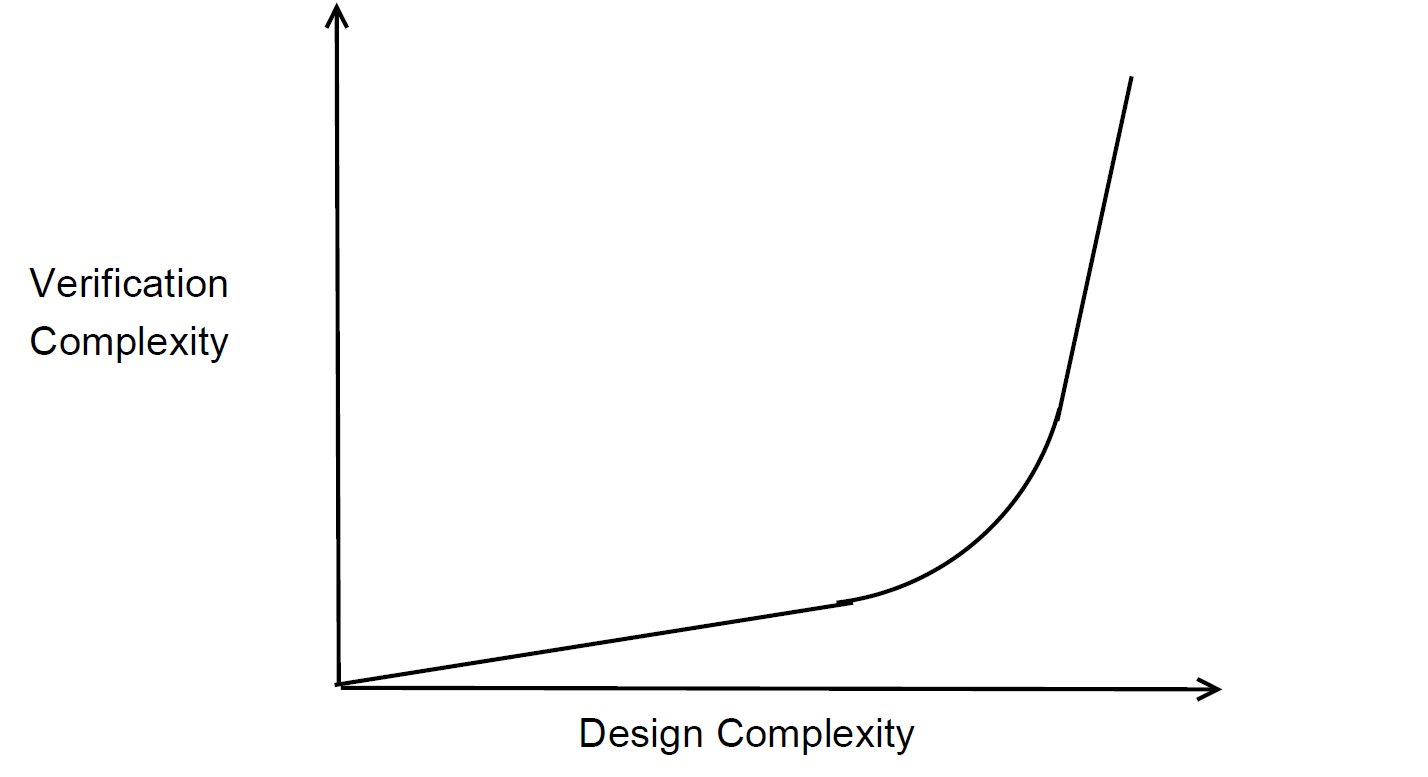
\includegraphics[scale = 0.5]{fv_graph.PNG}
    \caption{Design vs. Verification Complexity}
    \label{fig:fv_graph}
\end{figure}

\section{Hardware Design Overview}

Lorem ipsum dolor sit amet, consectetur adipiscing elit. Duis tincidunt eros ut dictum tempor. Proin rhoncus elementum mauris, ac bibendum quam. Sed eget nisi non arcu malesuada pulvinar a at ipsum. Curabitur ante quam, aliquet id purus ac, interdum semper odio. Suspendisse potenti. Aliquam rhoncus massa consectetur faucibus condimentum. Sed euismod tellus eu mattis elementum. In nec laoreet ligula. Donec vel blandit ante. Mauris non ligula non justo venenatis rhoncus. In quis auctor ipsum, in mattis lacus. In vitae lectus sodales arcu iaculis bibendum. Fusce ornare at ex vitae ultricies.

Nullam sagittis maximus leo, sit amet dictum neque suscipit at. Proin sagittis mollis mi, at ornare ligula ornare nec. Donec et pulvinar mi. Nulla ac semper dui, id mollis ante. Nam cursus vel tellus quis maximus. Vestibulum quis nunc sit amet felis mollis facilisis sed a sapien. Sed sit amet nisi velit. Mauris tellus arcu, commodo in feugiat in, porttitor vitae urna. Vivamus in aliquet elit. Nunc quis dui massa. Morbi blandit fringilla dui et fermentum. Nulla facilisi. Aenean et dui turpis. Mauris tempor diam ac mi scelerisque lacinia.

\subsection{Formal verification}
\begin{table}[H]
    \centering
    \begin{tabular}{| l | l | l | l | l |}
    \hline
    $k$ & $t_1$ & $t_2$ & $t_3$ & $t_4$ \\ \hline
    2 & 0.002 & 0.003 & 0.007 & 0.005 \\ \hline
    4 & 0.005 & 5.820 & 0.024 & 5.824 \\ \hline
    8 & 0.027 & 9.103 & 0.206 & 9.111 \\ \hline
    12 & 0.120 & 23.137 & 0.641 & 23.158 \\ \hline
    16 & 0.400 & 42.915 & 1.782 & 42.981 \\ \hline
    18 & 0.647 & 48.964 & 2.479 & 49.060  \\ \hline
    28 & 6.329 & 288.448 & 26.707  & 289.860\\ \hline
    32 & 12.119 & 368.319 & 44.965 & 370.579 \\ \hline
    56 & 292.203 & 980.283 & 1221.654 & 1040.504 \\ \hline
    64 & 577.162 & 16.049 & 28.597 & 20.147 \\
    \hline
    \end{tabular}
    \caption{Single-fix rectification of integer multiplier against polynomial specification. Time in seconds; k = Datapath size, $t_1$ = verification time, $t_2$ = time to find potentially rectifiable nets , $t_3$ = time for rectification check, $t_4$ = time to compute rectification function. Time Out = 10800 seconds.}
    \label{tb:tb1}
\end{table}
It subsequently describes how to select a net which admits single-fix rectification. Chapter \ref{ch:rectfunc} describes a procedure to compute a suitable rectification polynomial which, when implemented \ref{tb:tb1}

\section{Formal verification of integer arithmetic circuits}

Nullam sagittis maximus leo, sit amet dictum neque suscipit at. Proin sagittis mollis mi, at ornare ligula ornare nec. Donec et pulvinar mi. Nulla ac semper dui, id mollis ante. Nam cursus vel tellus quis maximus. Vestibulum quis nunc sit amet felis mollis facilisis sed a sapien. Sed sit amet nisi velit. Mauris tellus arcu, commodo in feugiat in, porttitor vitae urna. Vivamus in aliquet elit. Nunc quis dui massa. Morbi blandit fringilla dui et fermentum. Nulla facilisi. Aenean et dui turpis. Mauris tempor diam ac mi scelerisque lacinia.

\section{Thesis Organization}
Lorem ipsum dolor sit amet, consectetur adipiscing elit. Duis tincidunt eros ut dictum tempor. Proin rhoncus elementum mauris, ac bibendum quam. Sed eget nisi non arcu malesuada pulvinar a at ipsum. Curabitur ante quam, aliquet id purus ac, interdum semper odio. Suspendisse potenti. Aliquam rhoncus massa consectetur faucibus condimentum. Sed euismod tellus eu mattis elementum. In nec laoreet ligula. Donec vel blandit ante. Mauris non ligula non justo venenatis rhoncus. In quis auctor ipsum, in mattis lacus. In vitae lectus sodales arcu iaculis bibendum. Fusce ornare at ex vitae ultricies \ref{ch:rectfunc}.

Nullam sagittis maximus leo, sit amet dictum neque suscipit at. Proin sagittis mollis mi, at ornare ligula ornare nec. Donec et pulvinar mi. Nulla ac semper dui, id mollis ante. Nam cursus vel tellus quis maximus. Vestibulum quis nunc sit amet felis mollis facilisis sed a sapien. Sed sit amet nisi velit. Mauris tellus arcu, commodo in feugiat in, porttitor vitae urna. Vivamus in aliquet elit. Nunc quis dui massa. Morbi blandit fringilla dui et fermentum. Nulla facilisi. Aenean et dui turpis. Mauris tempor diam ac mi scelerisque lacinia.
\chapter{Computing Rectification function}
\label{ch:rectfunc}
Lorem ipsum dolor sit amet, consectetur adipiscing elit. Duis tincidunt eros ut dictum tempor. Proin rhoncus elementum mauris, ac bibendum quam. Sed eget nisi non arcu malesuada pulvinar a at ipsum. Curabitur ante quam, aliquet id purus ac, interdum semper odio. Suspendisse potenti. Aliquam rhoncus massa consectetur faucibus condimentum. Sed euismod tellus eu mattis elementum. In nec laoreet ligula. Donec vel blandit ante. Mauris non ligula non justo venenatis rhoncus. In quis auctor ipsum, in mattis lacus. In vitae lectus sodales arcu iaculis bibendum. Fusce ornare at ex vitae ultricies.

Nullam sagittis maximus leo, sit amet dictum neque suscipit at. Proin sagittis mollis mi, at ornare ligula ornare nec. Donec et pulvinar mi. Nulla ac semper dui, id mollis ante. Nam cursus vel tellus quis maximus. Vestibulum quis nunc sit amet felis mollis facilisis sed a sapien. Sed sit amet nisi velit. Mauris tellus arcu, commodo in feugiat in, porttitor vitae urna. Vivamus in aliquet elit. Nunc quis dui massa. Morbi blandit fringilla dui et fermentum. Nulla facilisi. Aenean et dui turpis. Mauris tempor diam ac mi scelerisque lacinia.

\section{Problem Statement}

\begin{Example}
Consider a buggy 2-bit multiplier in Fig. \ref{fig:mult2_b2}. 

\begin{figure}[H]
    \centering
    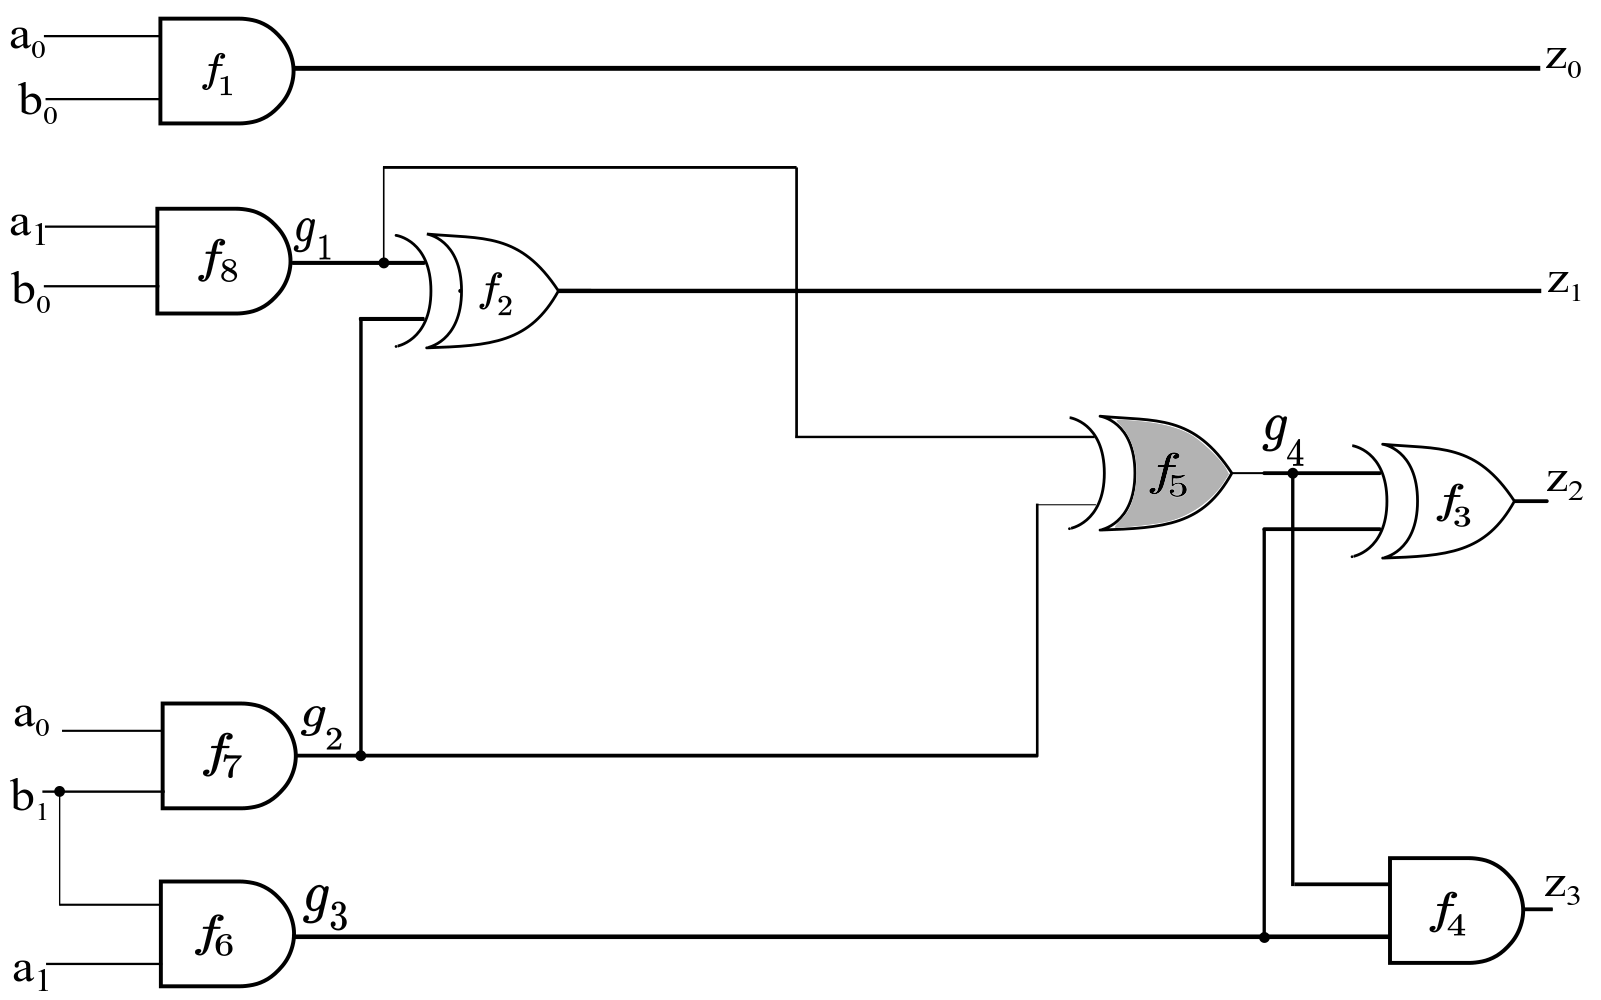
\includegraphics[scale = 0.2]{mult2_b.png}
    \caption{2-bit Integer multiplier with a bug. The AND gate at $g_4$ replaced by an XOR gate.}
    \label{fig:mult2_b2}
\end{figure}

\end{Example}

\section{Computing rectification function}

LLorem ipsum dolor sit amet, consectetur adipiscing elit. Duis tincidunt eros ut dictum tempor. Proin rhoncus elementum mauris, ac bibendum quam. Sed eget nisi non arcu malesuada pulvinar a at ipsum. Curabitur ante quam, aliquet id purus ac, interdum semper odio. Suspendisse potenti. Aliquam rhoncus massa consectetur faucibus condimentum. Sed euismod tellus eu mattis elementum. In nec laoreet ligula. Donec vel blandit ante. Mauris non ligula non justo venenatis rhoncus. In quis auctor ipsum, in mattis lacus. In vitae lectus sodales arcu iaculis bibendum. Fusce ornare at ex vitae ultricies.

Nullam sagittis maximus leo, sit amet dictum neque suscipit at. Proin sagittis mollis mi, at ornare ligula ornare nec. Donec et pulvinar mi. Nulla ac semper dui, id mollis ante. Nam cursus vel tellus quis maximus. Vestibulum quis nunc sit amet felis mollis facilisis sed a sapien. Sed sit amet nisi velit. Mauris tellus arcu, commodo in feugiat in, porttitor vitae urna. Vivamus in aliquet elit. Nunc quis dui massa. Morbi blandit fringilla dui et fermentum. Nulla facilisi. Aenean et dui turpis. Mauris tempor diam ac mi scelerisque lacinia.

\begin{equation}
\label{eq:eqn1}
    f \in \langle f_1,\dots,f_{i-1},\boldsymbol{f_i: x_i - U},f_{i+1},\dots,f_s,x_1^2-x_1,\dots,x_n^2-x_n \rangle
\end{equation}

Lorem ipsum dolor sit amet, consectetur adipiscing elit. Duis tincidunt eros ut dictum tempor. Proin rhoncus elementum mauris, ac bibendum quam. Sed eget nisi non arcu malesuada pulvinar a at ipsum. Curabitur ante quam, aliquet id purus ac, interdum semper odio. Suspendisse potenti. Aliquam rhoncus massa consectetur faucibus condimentum. Sed euismod tellus eu mattis elementum. In nec laoreet ligula. Donec vel blandit ante. Mauris non ligula non justo venenatis rhoncus. In quis auctor ipsum, in mattis lacus. In vitae lectus sodales arcu iaculis bibendum. Fusce ornare at ex vitae ultricies.

Nullam sagittis maximus leo, sit amet dictum neque suscipit at. Proin sagittis mollis mi, at ornare ligula ornare nec. Donec et pulvinar mi. Nulla ac semper dui, id mollis ante. Nam cursus vel tellus quis maximus. Vestibulum quis nunc sit amet felis mollis facilisis sed a sapien. Sed sit amet nisi velit. Mauris tellus arcu, commodo in feugiat in, porttitor vitae urna. Vivamus in aliquet elit. Nunc quis dui massa. Morbi blandit fringilla dui et fermentum. Nulla facilisi. Aenean et dui turpis. Mauris tempor diam ac mi scelerisque lacinia.

\subsection{Procedure to compute rectification function}
\vspace{2mm}
\begin{table}[ht]
    \centering
    \begin{tabular}{|c|c|c|} \hline
      $a_0,a_1,a_2,b_0,b_1,b_2$ & $h_i$ & $h_i'$ \\ \hline
       0,0,0,0,0,0 & -12 & 1\\ \hline
       0,0,0,0,0,1 & -12 & 1\\ \hline
       0,0,0,0,1,0 & -12 & 1\\ \hline
       0,1,0,0,0,1 & 0 & $-\frac{1}{3}$\\ \hline
       0,1,0,0,1,0 & 0 & $\frac{1}{3}$\\ \hline
       0,1,0,0,1,1 & 0 & -1 \\ \hline
    \end{tabular}
    \caption{Evaluating $h_i$ and $h_i'$}
    \label{tab:quosol}
\end{table}

In order to conserve space, Table \ref{tab:quosol} shows the data for only some input patterns. We make some observations based on the contents of this table. 

\section{Conclusion}
Lorem ipsum dolor sit amet, consectetur adipiscing elit. Duis tincidunt eros ut dictum tempor. Proin rhoncus elementum mauris, ac bibendum quam. Sed eget nisi non arcu malesuada pulvinar a at ipsum. Curabitur ante quam, aliquet id purus ac, interdum semper odio. Suspendisse potenti. Aliquam rhoncus massa consectetur faucibus condimentum. Sed euismod tellus eu mattis elementum. In nec laoreet ligula. Donec vel blandit ante. Mauris non ligula non justo venenatis rhoncus. In quis auctor ipsum, in mattis lacus. In vitae lectus sodales arcu iaculis bibendum. Fusce ornare at ex vitae ultricies.

Nullam sagittis maximus leo, sit amet dictum neque suscipit at. Proin sagittis mollis mi, at ornare ligula ornare nec. Donec et pulvinar mi. Nulla ac semper dui, id mollis ante. Nam cursus vel tellus quis maximus. Vestibulum quis nunc sit amet felis mollis facilisis sed a sapien. Sed sit amet nisi velit. Mauris tellus arcu, commodo in feugiat in, porttitor vitae urna. Vivamus in aliquet elit. Nunc quis dui massa. Morbi blandit fringilla dui et fermentum. Nulla facilisi. Aenean et dui turpis. Mauris tempor diam ac mi scelerisque lacinia. 

\chapter{Conclusions and future work}
\label{ch:conclusion}

Lorem ipsum dolor sit amet, consectetur adipiscing elit. Duis tincidunt eros ut dictum tempor. Proin rhoncus elementum mauris, ac bibendum quam. Sed eget nisi non arcu malesuada pulvinar a at ipsum. Curabitur ante quam, aliquet id purus ac, interdum semper odio. Suspendisse potenti. Aliquam rhoncus massa consectetur faucibus condimentum. Sed euismod tellus eu mattis elementum. In nec laoreet ligula. Donec vel blandit ante. Mauris non ligula non justo venenatis rhoncus. In quis auctor ipsum, in mattis lacus. In vitae lectus sodales arcu iaculis bibendum. Fusce ornare at ex vitae ultricies.

\section{Future Work}
Lorem ipsum dolor sit amet, consectetur adipiscing elit. Duis tincidunt eros ut dictum tempor. Proin rhoncus elementum mauris, ac bibendum quam. Sed eget nisi non arcu malesuada pulvinar a at ipsum. Curabitur ante quam, aliquet id purus ac, interdum semper odio. Suspendisse potenti. Aliquam rhoncus massa consectetur faucibus condimentum. Sed euismod tellus eu mattis elementum. In nec laoreet ligula. Donec vel blandit ante. Mauris non ligula non justo venenatis rhoncus. In quis auctor ipsum, in mattis lacus. In vitae lectus sodales arcu iaculis bibendum. Fusce ornare at ex vitae ultricies.

\subsection{Computing multiple rectification functions}

Lorem ipsum dolor sit amet, consectetur adipiscing elit. Duis tincidunt eros ut dictum tempor. Proin rhoncus elementum mauris, ac bibendum quam. Sed eget nisi non arcu malesuada pulvinar a at ipsum. Curabitur ante quam, aliquet id purus ac, interdum semper odio. Suspendisse potenti. Aliquam rhoncus massa consectetur faucibus condimentum. Sed euismod tellus eu mattis elementum. In nec laoreet ligula. Donec vel blandit ante. Mauris non ligula non justo venenatis rhoncus. In quis auctor ipsum, in mattis lacus. In vitae lectus sodales arcu iaculis bibendum. Fusce ornare at ex vitae ultricies. Fig. \ref{fig:2bit_redbI}. 

\begin{figure}[htp]
    \centering
    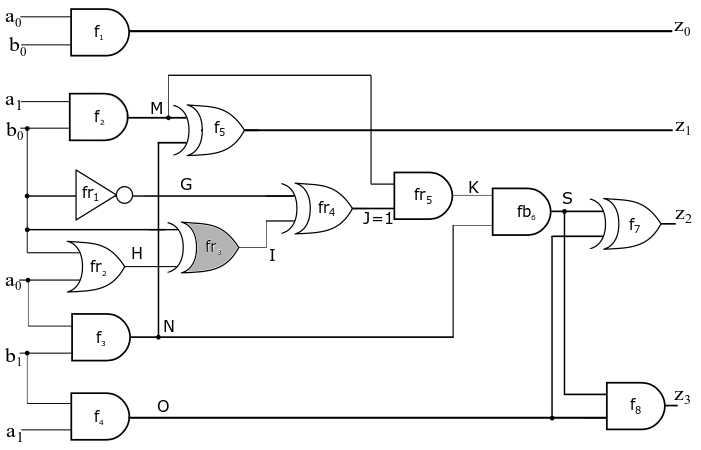
\includegraphics[scale = 0.5]{int2_red_bI.png}
    \caption{2-bit integer multiplier with redundancy. Bug at $I$.}
    \label{fig:2bit_redbI}
\end{figure}

The procedure to compute a rectification polynomial is applied and the polynomial $I = b_0$ is computed.

\subsection{Dependency constrained rectification function}

Lorem ipsum dolor sit amet, consectetur adipiscing elit. Duis tincidunt eros ut dictum tempor. Proin rhoncus elementum mauris, ac bibendum quam. Sed eget nisi non arcu malesuada pulvinar a at ipsum. Curabitur ante quam, aliquet id purus ac, interdum semper odio. Suspendisse potenti. Aliquam rhoncus massa consectetur faucibus condimentum. Sed euismod tellus eu mattis elementum. In nec laoreet ligula. Donec vel blandit ante. Mauris non ligula non justo venenatis rhoncus. In quis auctor ipsum, in mattis lacus. In vitae lectus sodales arcu iaculis bibendum. Fusce ornare at ex vitae ultricies.

\subsection{Impact of term orders on efficiency}

Lorem we discuss the limitation of \Grobner Basis reduction with Reverse Topological Term Order (RTTO) imposed on the variables. We witness the problem of variable explosion. Consider the example below, where \Grobner Basis reduction is performed with a forward topology based term order. 

\begin{Example}
Lorem ipsum dolor sit amet, consectetur adipiscing elit. Duis tincidunt eros ut dictum tempor. Proin rhoncus elementum mauris, ac bibendum quam. Sed eget nisi non arcu malesuada pulvinar a at ipsum. Curabitur ante quam, aliquet id purus ac, interdum semper odio. Suspendisse potenti. Aliquam rhoncus massa consectetur faucibus condimentum. Sed euismod tellus eu mattis elementum. In nec laoreet ligula. Donec vel blandit ante. Mauris non ligula non justo venenatis rhoncus. In quis auctor ipsum, in mattis lacus. In vitae lectus sodales arcu iaculis bibendum. Fusce ornare at ex vitae ultricies.
\end{Example}

\subsection{Multi-fix rectification}

Not all the bugs that may be present in a circuit can be rectified at a single location. Some bugs can be rectified only by the implementation of multiple functions at multiple nets in the circuit. 



\numberofappendices = 0

\bibliographystyle{ieee}
\bibliography{vikas}

\end {document}
